% Intended LaTeX compiler: pdflatex
\documentclass[bigger]{beamer}
\usepackage[utf8]{inputenc}
\usepackage[T1]{fontenc}
\usepackage{graphicx}
\usepackage{longtable}
\usepackage{wrapfig}
\usepackage{rotating}
\usepackage[normalem]{ulem}
\usepackage{amsmath}
\usepackage{amssymb}
\usepackage{capt-of}
\usepackage{hyperref}
\mode<beamer>{\usetheme{Madrid}}
\mode<beamer>{\usepackage{amsmath}}
\usetheme{default}
\author{Konstantinos Papadimos}
\date{}
\title{Presentation draft}
\hypersetup{
 pdfauthor={Konstantinos Papadimos},
 pdftitle={Presentation draft},
 pdfkeywords={},
 pdfsubject={},
 pdfcreator={Emacs 28.2 (Org mode 9.5.5)}, 
 pdflang={English}}
\begin{document}

\maketitle

\section{Introductory stuff, Detectros and Particle physics}
\label{sec:org1fd9538}
\begin{frame}[label={sec:org3b8dca7}]{The CMS Experiment overview}
The CMS detector at the LHC
\begin{figure}[hb]
\centering
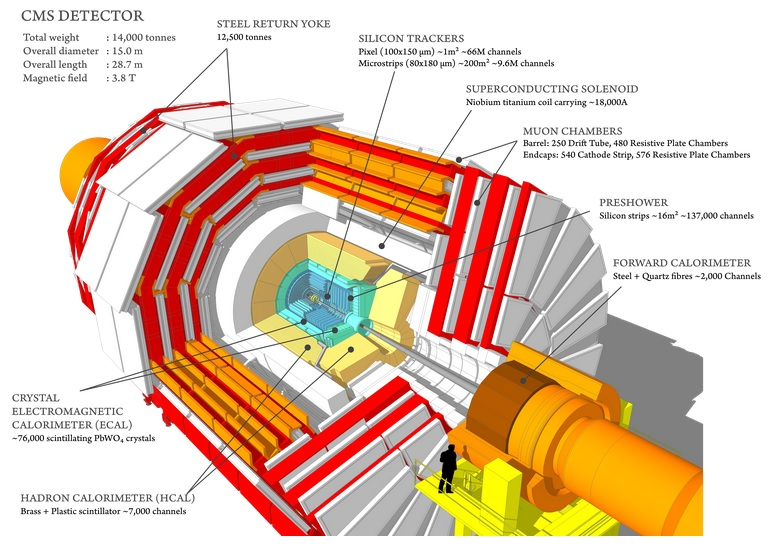
\includegraphics[width=0.7 \textwidth, ext=.png type=jpg]{/home/kpapad/UG_thesis/Thesis/Dissertation/src/figures/cms_detector.jpg}
\end{figure}
\end{frame}

\begin{frame}[label={sec:org2db6cf2}]{Coordinates at the CMS}
Given the solenoid geometry of the CMS detector, it is more convenient to use a spherical type of coordinates\(\left(r, \phi, \theta \right)\).
\begin{equation}
\begin{matrix}
p_{x} = P_{T}\cos{\phi} \\
p_{y} = P_{T}\sin{\phi} \\
p_{z} = P_{T}\sinh{\eta}\\
|\vec{P}| = P_{T}\cosh{\eta} 
\end{matrix}
\end{equation}
\(\phi \in \left [ 0, 2\pi \right]\)the azimuthal angle, and \(\eta\in \left [ -\infty, +\infty \right ]\) is defined as:
\begin{equation}
\eta \equiv -\ln{\left [ \tan\left (\frac{\theta}{2} \right ) \right]  }
\end{equation}
\end{frame}

\begin{frame}[label={sec:org4290248}]{Decays \& Resonances}
Not every particle can be detected by the CMS detector(i.e neutrinos)
\begin{columns}
\begin{column}{0.5\columnwidth}
\begin{itemize}
\item Detectable Decay Products \(\rightarrow\) Resonance
\end{itemize}
\begin{center}
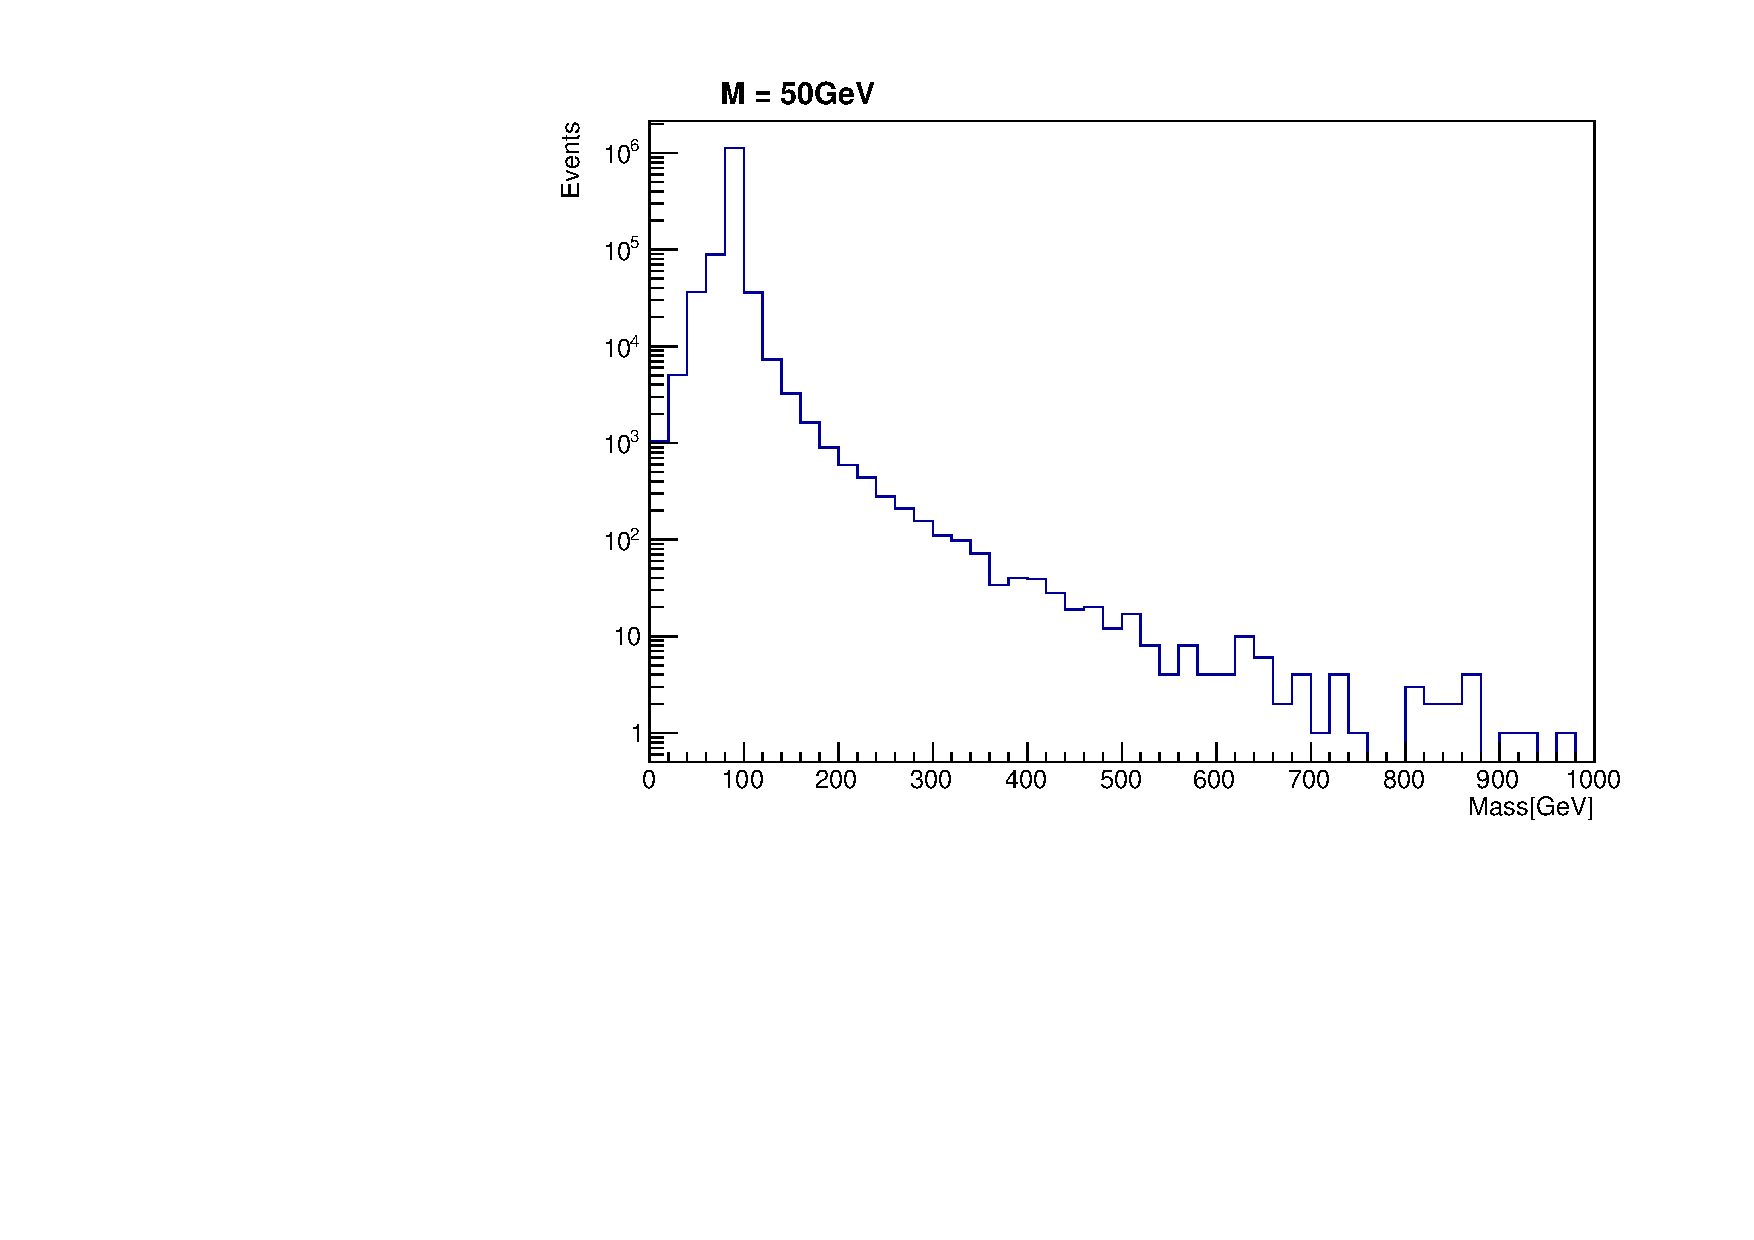
\includegraphics[width=0.8\textwidth]{/home/kpapad/UG_thesis/Thesis/Analysis/out/Plots/DYJetsM50_MassHist.pdf}
\end{center}
\end{column}

\begin{column}{0.5\columnwidth}
\begin{itemize}
\item Non Detectable Decay Products \(\rightarrow\) Not a resonance
\end{itemize}
\begin{center}
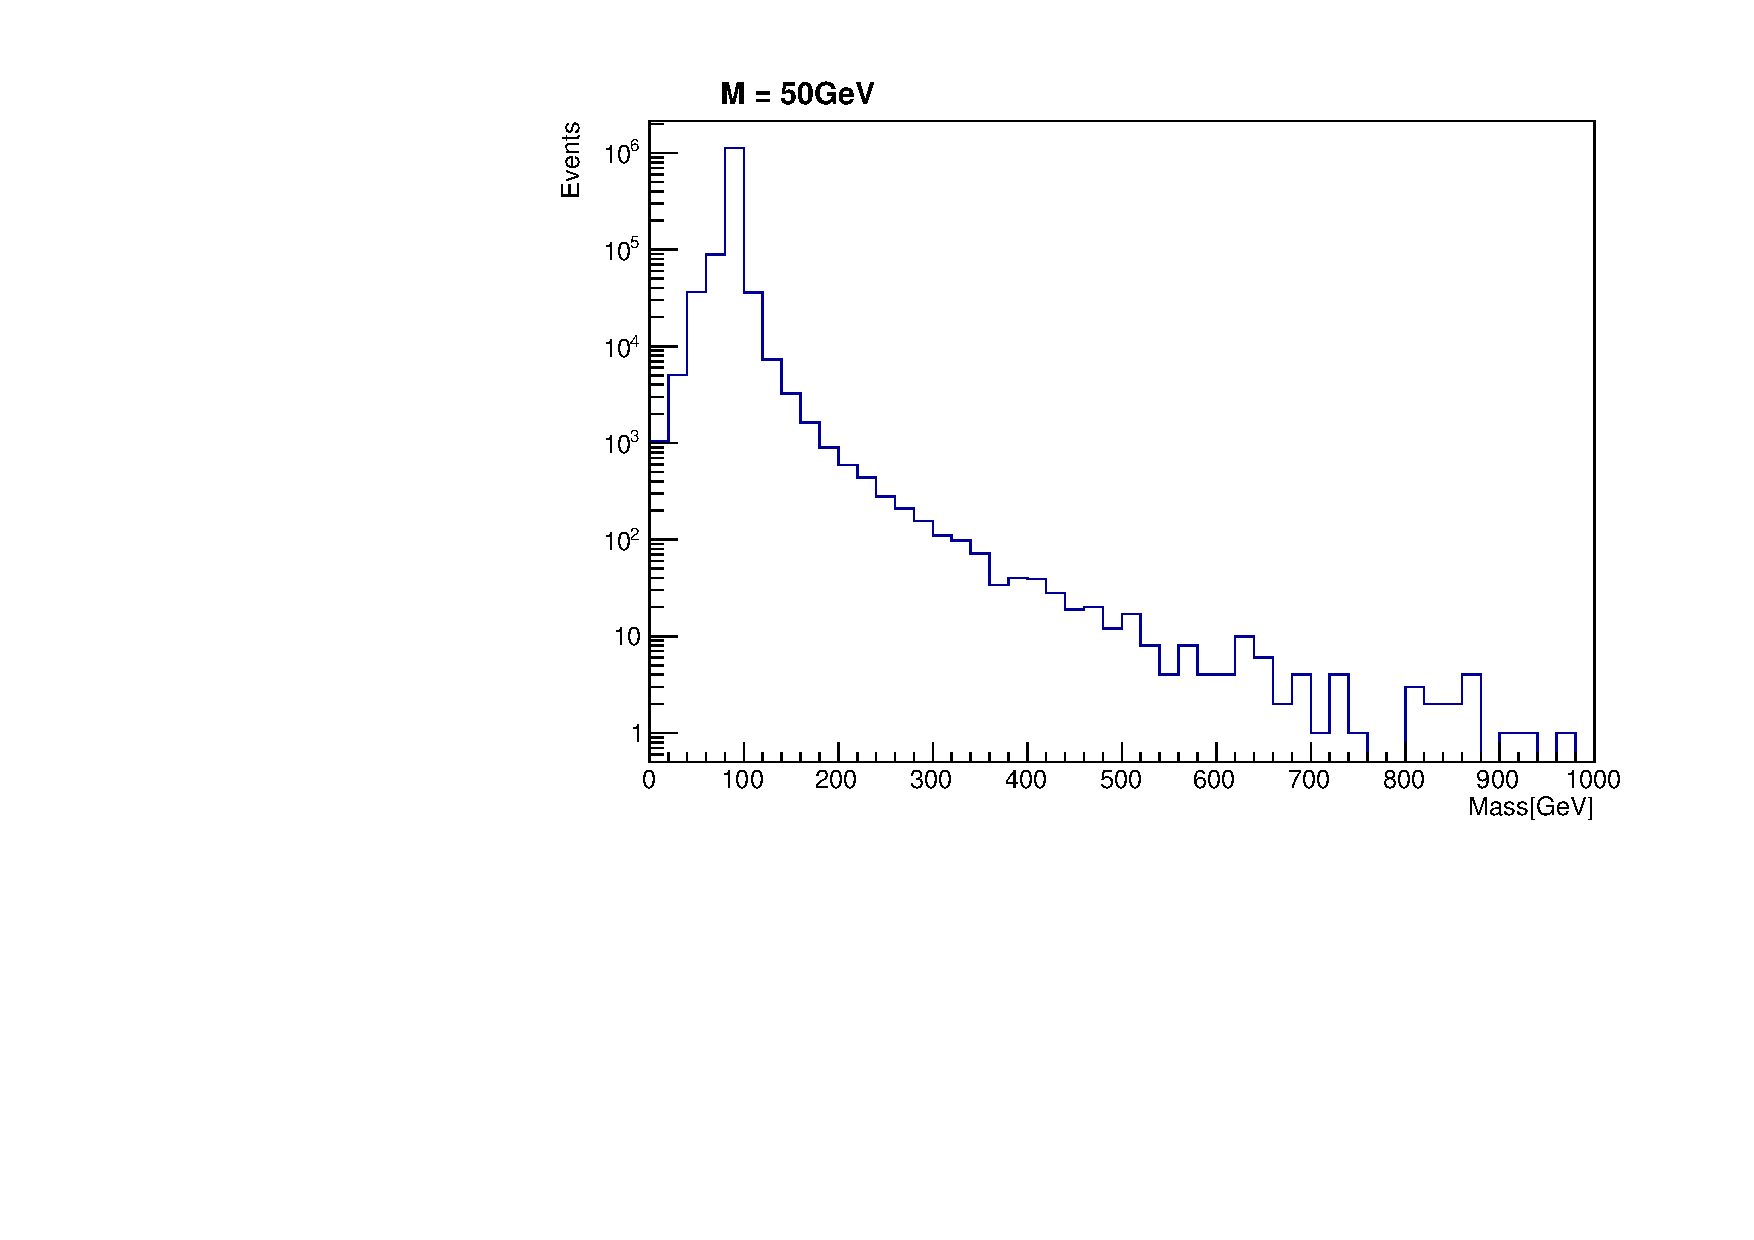
\includegraphics[width=.9\linewidth]{/home/kpapad/UG_thesis/Thesis/Analysis/out/Plots/DYJetsM50_MassHist.pdf}
\end{center}
\end{column}
\end{columns}
\end{frame}

\begin{frame}[label={sec:org0112bcc}]{Calibration and energy scale uncertainties}
\begin{itemize}
\item Calibration process adjusts energy scale and resolution to match well-known resonances (Z boson, J/psi meson) in data and simulation,
\end{itemize}
\begin{itemize}
\item Imperfect agreement due to subdetector complexities and nonlinear effects
\end{itemize}
\begin{block}{How do analysis techniques respond to energy scale uncertainties ?}
Our work will focus on the effects that energy scale uncertainties have, on a traditional fit-based analysis and a more modern Boosted Decision Tree-based analysis, using the generic diobject production process as the working example.
\end{block}
\end{frame}
\section{Analysis techniqies}
\label{sec:org761ad25}
\begin{frame}[label={sec:org5651aca}]{BDT 1: Supervised Learning}
\alert{Supervised learning}:
\begin{itemize}
\item The model is trained using training data
\item The trained model is tested using testing data
\item If we like the resulting model, we apply it!
\end{itemize}

\alert{but what is this model?}
\begin{itemize}
\item A function that given the input feautres x, it returns the probability x beeing class A
\item The goal of the training is to minimize the difference between the predicted output \(y_{i} \in [0, 1]\) and the real output \(\hat{y_{i}} = 0\text{ class B, or }\hat{y_{i}} = 1\text{ class A}\)
\end{itemize}
\end{frame}
\begin{frame}[label={sec:org7dc6970}]{BDT 2a: Boosted decision trees}
In this study the model of choice is Boosted Decision Trees(BDT).
\begin{itemize}
\item It classifies data using decision tree models
\end{itemize}
\begin{figure}[h]
\centering
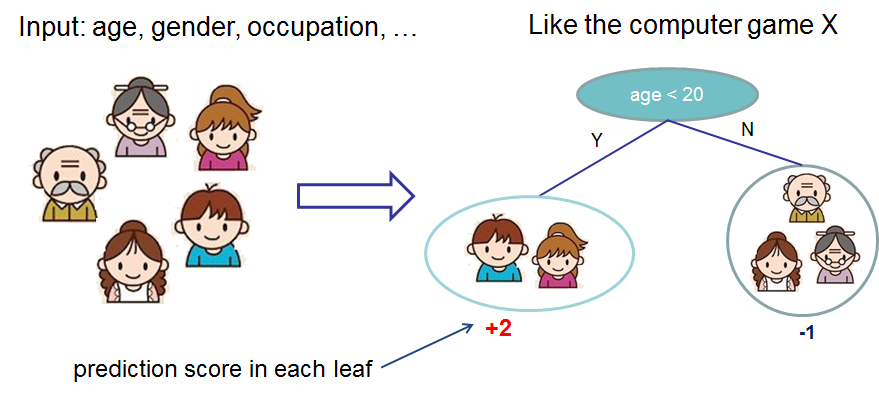
\includegraphics[width=0.85 \textwidth, ext=.png type=png]{/home/kpapad/UG_thesis/Thesis/Dissertation/Presentation/figures/cart.png}
\end{figure}
\end{frame}
\begin{frame}[label={sec:org26e8efc}]{BDT 2b: Boosted Decision Trees}
Usually only one tree is not power full enough --> Use  more trees in additive manner(Boosting)
\begin{figure}[h]
\centering
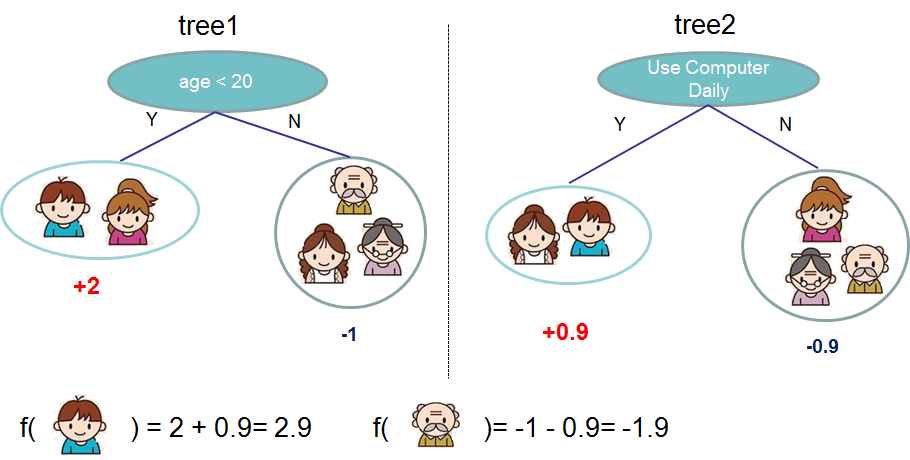
\includegraphics[width=0.85 \textwidth, ext=.png type=png]{/home/kpapad/UG_thesis/Thesis/Dissertation/Presentation/figures/twocart.png}
\end{figure}
\end{frame}
\begin{frame}[label={sec:org45bd927}]{BDT 3a: Signal from Background Separation}
\alert{In our case}:
\begin{itemize}
\item Signal: a resonant decay Y->xx
\item Background: a non resonant process
\end{itemize}
\alert{How to separate them?}
\begin{itemize}
\item Plot the number of Signal and Background events per BDT score --> BDT histogram
\end{itemize}
\end{frame}
\begin{frame}[label={sec:orga2d6ed6}]{BDT 3b: Signal from background separation}
Where should we place the cut in order to accpet most most of the  signal while rejecting most of background?
\begin{figure}[hb]
\centering
\includegraphics[page=2, width=0.85 \textwidth, ext=.png type=jpg]{/home/kpapad/UG_thesis/Thesis/Bdt/out/Plots/WPhiJets_M60M5080DeltasPConf12BDTplot.pdf}
\end{figure}
\end{frame}
\begin{frame}[label={sec:orgfd171a4}]{Fit based signal from background separation}
Fit the mass spectrum \ldots{}
\begin{figure}[hb]
\centering
\includegraphics[page=2, width=0.5 \textwidth, ext=.png type=jpg]{/home/kpapad/UG_thesis/Thesis/Analysis/src/WPhiJets_M60M5080_SampleFitWArrows.pdf}
\end{figure}
\end{frame}
\begin{frame}[label={sec:org9e3227f}]{Fit based signal from background separation}
\ldots{} and decompose it to a background component \ldots{}
\begin{figure}[hb]
\centering
\includegraphics[page=3, width=0.5 \textwidth, ext=.png type=jpg]{/home/kpapad/UG_thesis/Thesis/Analysis/src/WPhiJets_M60M5080_SampleFitWArrows.pdf}
\end{figure}
\end{frame}
\begin{frame}[label={sec:org40139d9}]{Fit based signal from background separation}
\ldots{} and a signal component
\begin{figure}[hb]
\centering
\includegraphics[page=4, width=0.5 \textwidth, ext=.png type=jpg]{/home/kpapad/UG_thesis/Thesis/Analysis/src/WPhiJets_M60M5080_SampleFitWArrows.pdf}
\end{figure}
\end{frame}
\begin{frame}[label={sec:org63a4d5b}]{Fit based signal from background separation}
Then we can count the signal and background events, in a region of interest \(I\):
\begin{align}
O &= \int_{I} observation(x) dx \\
B &= \int_{I} bkg(x) dx\\
S &= O - B
\end{align}
\end{frame}
\begin{frame}[label={sec:org51c3761}]{Statistical interpretation of results}
\alert{Are the signal events we counted, statistically significant?}
\begin{itemize}
\item We use the following metric:
\end{itemize}
\begin{equation}
\text{Significance} = \frac{Signal}{\sqrt{Background}}
\end{equation}
\begin{itemize}
\item The selected regions of interest both in BDT and Fit based analysis, are those that maximize the significance.
\end{itemize}
\end{frame}

\section{Analysis}
\label{sec:org05ae1c6}
\begin{frame}[label={sec:orgd974eb2}]{Energy scale uncertainties}
How we implemented the smearing in our data set. How do we proceed from that, how many smearing cases. 
\end{frame}
\begin{frame}[label={sec:org009670c}]{BDT approach 1}
Train Testing application set. Summarize the number of events. Explain that in order to compare apples to apples, we will be analyzing the application set from now on.
\end{frame}
\begin{frame}[label={sec:orgbc17049}]{BDT approach 2}
Application summarize the results 
\end{frame}
\begin{frame}[label={sec:org35b9f4a}]{Fit based approach 1}
Show the mass spectrum that will be fitted 
\end{frame}
\begin{frame}[label={sec:orge0b214a}]{Fit based approach 2}
discuss bkg fit is kept constnat throughout the analysis. discus signal fitting, show the plots( I will probably need more than one slide) at this part talk about the fact that after \(20\%\) the fit based technique fails. 
\end{frame}
\begin{frame}[label={sec:org311865b}]{Fit based approach 2}
Present the significances.
\end{frame}
\section{Results}
\label{sec:org157a95e}
\begin{frame}[label={sec:orgdf3f139}]{Results 1}
Compare the BDT and FIt in terms of significance and robustness. Comment that even though fit based achieves a higher significance in the 0 smearing case, it is not as robust as bdt, it completelly fails at extreme cases of smearing,. BDT is more robust 
\end{frame}
\begin{frame}[label={sec:org53992a3}]{Results 2}
Try to explain that bdt uses not only energy related features (Pts) but also geometrical ones, which do not get affected by smearing. Therefore, more stabillity to smearing. Nevertheless robustness does not mean greateer classification "power"(how many events got classified correctly and how manny didn't) -->Outlooks for better training methods in other to increase classification power.   
\end{frame}
\section{Unused stuff}
\label{sec:org810ab9a}
\begin{frame}[label={sec:org247ee24}]{Unused stuff}
\alert{Welcome to the backup slides!}
\end{frame}
\begin{frame}[label={sec:org2f9ca01}]{Resonance text}
and therefore, the invariant mass calculation from the detected particles of such events will not result in a peak at the mass spectrum(Non resonant proces). Even though in decays where  the poducts are detectable particles, the invariant mass calculation leads to a peak in the mass spectrum(resonant decays). In the present work we are interested in the later.
\end{frame}
\end{document}